%!TEX root = ../thesis.tex
% **************************** Define Graphics Path **************************
\ifpdf
\graphicspath{{Chapter4/Figs/Raster/}{Chapter4/Figs/PDF/}{Chapter4/Figs/}}
\else
\graphicspath{{Chapter4/Figs/Vector/}{Chapter4/Figs/}}
\fi

%*******************************************************************************
%****************************** Fourth Chapter *********************************
%*******************************************************************************

\chapter{Methodology}
\label{chapter4}
This chapter presents the computational method developed in this thesis. We start by introducing each component of the method separately. We discuss neural networks, automatic differentiation, gradient-based optimisation, and importance sampling. Finally, we present the actual implementation in \emph{JAX}, and discuss computational considerations and intricacies of thereof.

\section{Neural Networks} % ~150 words
\subsection{The Multilayer Perceptron}
The \textbf{multilayer perceptron} (MLP), also referred to as a \textbf{deep feedforward network} or simply a \textbf{deep neural network} (DNN), is the paradigmatic model of deep learning and serves as a foundation for more advanced models. In essence it is nothing more than a mapping of inputs to outputs
\begin{equation}
	f(\mathbf{x}; ~\theta): \mathbb{R}^\text{in} \rightarrow \mathbb{R}^{\text{out}},
\end{equation}
which is structured in a certain way and depends on parameters $\theta$. The mapping is a composition of vector-valued functions $f$ which are called \emph{layers} of the network, and with each layer we associate variational parameters $\mathbf{w}$, or simply the weights. The MLP can be described with a directed acyclic graph which details the compositions of the layers. The simplest and most common is a chain of compositions, in Fig~\ref{fig:mlp}b, 
\begin{equation}
f_{\text{MLP}} = \left(f^{(n)} \circ f^{(n-1)} \circ \cdots \circ f^{(2)} \circ f^{(1)} \right)(\mathbf{x}),
\end{equation}
where the input $\textbf{x}$ passes through \emph{hidden} layers before the \emph{output} layer outputs the result. The length of this chain is the \emph{depth} of the network, and the dimensionality of hidden layers is the \emph{width} of the network. We can interpret each transformation $f^{(i)}$ as consisting of a unit/node/neuron for each input dimension, which is a vector-to-scalar transformation, Fig~\ref{fig:mlp}a.
\begin{figure}[H]
	\centering
	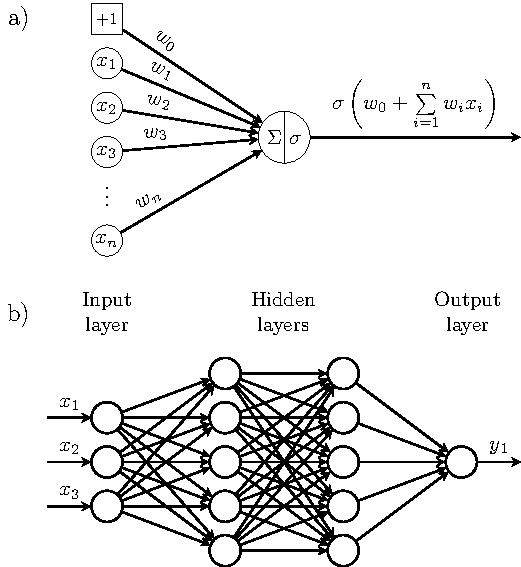
\includegraphics[width=\linewidth]{Chapter4/Figs/Vector/mlp.pdf}
	\caption[Multilayer Perceptron]{\textbf{Multilayer Perceptron.} A node outputs the activation function $\sigma$ evaluated at the weighted average of outputs from the previous layer and bias (\textbf{a}). A MLP with two hidden layers ($f^{(1)}: \mathbb{R}^3 \rightarrow \mathbb{R}^4$, $f^{(2)}: \mathbb{R}^4 \rightarrow \mathbb{R}^4$, $f^{(3)}: \mathbb{R}^4 \rightarrow \mathbb{R}$) in (\textbf{b}).}
	\label{fig:mlp}
\end{figure} 
\noindent
The simplest layer would be a linear one, composed of
\begin{equation}
f(\mathbf{x}; \mathbf{w}, b) = \mathbf{x}^\intercal \mathbf{w} + b.
\end{equation}
However, a linear neural network famously cannot learn the XOR function~\cite{minsky2017perceptrons}, and in practice a nonlinearity or \emph{activation} function $g(\cdot)$ is used in each node to bolster the network's representational power
\begin{equation}
f(\mathbf{x}; \mathbf{w}, b) = g\left(\mathbf{x}^\intercal \mathbf{w} + b\right).
\end{equation}
A variety of activations have been used, namely $\tanh(\cdot)$ and the logistic sigmoid $\sigma(\cdot)$, but have since been displaced by the use of the \textbf{rectified linear unit} or $\operatorname{ReLu}(\cdot)$, which is advantageous for training. For the output layer we will use the \emph{softplus}, which fulfils the requirement of being positive everywhere, Fig.~\ref{fig:activations}. A multilayer perceptron is a \textbf{universal function approximator}, meaning that it can approximate any Borel measurable function mapping from a finite-dimensional space to another with desired accuracy, if it has at least one hidden layer and sufficient hidden units~\cite{leshno1993multilayer}. While this means that a large enough network will be able do represent the rates, it provides no guarantee that learning the correct rates will be efficient or possible. 
\begin{figure}[H]
	\centering
	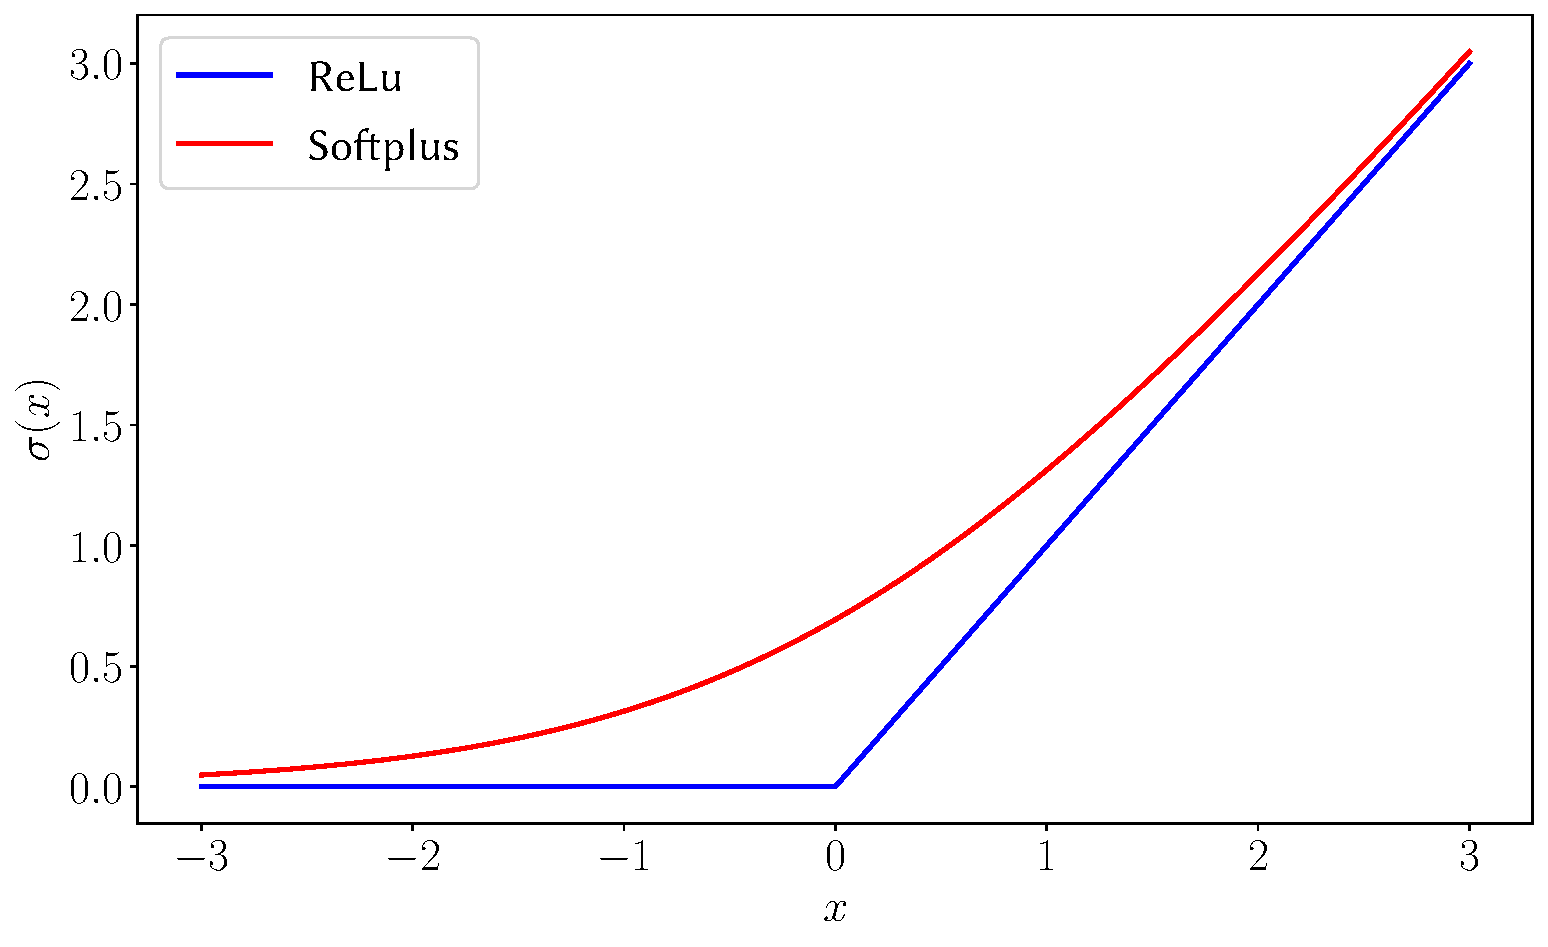
\includegraphics[width=0.7\linewidth]{Chapter4/Figs/Vector/activations}
	\caption[Activation functions]{\textbf{Activation functions.} $\operatorname{ReLu}$ and Softmax nonlinearities.}
	\label{fig:activations}
\end{figure}

\subsection{Convolutional Neural Networks}
\label{subsec:nn-cnn} 
Convolutional neural networks (CNN)~\cite{lecun1989generalization} make use of three powerful concepts to increase performance, \textbf{sparse interactions}, \textbf{parameter sharing} and \textbf{equivariant representations}~\cite{goodfellow2016deep}. At the core of a CNN is the {convolutional} layer, in which the input $I$ is convolved with the \textbf{kernel} $K$ as 
\begin{equation}
	\label{eq:convolution}
	S_{i,j} = (I * K)_{i,j} = \sum_m \sum_n I_{m,n} K_{i-m, j-n},
\end{equation}
in two dimensions, Fig.~\ref{fig:pcnn}a. Outputs of convolutions are referred to as \emph{feature maps}. In practice the kernel $K$ is much smaller than the input, meaning that each neuron is connected only to a small fraction of neurons in the previous layer. Hence the layers are sparsely connected in contrast to the fully connected layer, see Fig.~\ref{fig:pcnn}c. This decreases the number of weights and operations required. Moreover, the kernel is applied everywhere in the input, meaning the weights are shared across all connections and need to be learned for the whole input as opposed to every single position in the input. This makes the convolutional layer much more memory efficient than the fully connected layer. Moreover, the nature of convolution in eq.~\eqref{eq:convolution} means that the convolutional layer is equivariant to translation, i.e. a translation of the input results in the same translation of the output. Altogether, a convolutional layer is a transformation acting on a batch of examples $N_b$ with channels $N_c$
\begin{equation}
	f: \mathbb{R}^{(N_b, N_w, N_h, N_c)} \rightarrow \mathbb{R}^{(N_b, O_w, O_h, N_c)}.
\end{equation}
The output dimensions also depend on the \textbf{stride} (how quick the kernel travels)~$N_S$ and \textbf{padding}~$N_P$ (how much the dimension of input is increased), Fig.~\ref{fig:pcnn}a,
\begin{equation}
	O_{\text{out}} = \frac{N_{\text{in}}-N_K+2N_P}{N_S}+1.
\end{equation}
Alongside convolutional layers, CNNs often employ \emph{pooling} layers which downsample the input by combining a cluster of neurons into a single one. \emph{Max} and \emph{average} pooling are in common use, the pooling output is the max or average of the cluster respectively. A pooling layer can act globally, on the whole feature map, or locally. 

The models we are interested in will be image-to-image networks that preserve the input shape, as the outputs will represent the rates corresponding to adjacent states. In the Ising model, the output at $(i, j)$ is the rate associated with transition $s \rightarrow s^\prime$ where the spin at $(i, j)$ is flipped.
\subsubsection{Periodic CNN}
The simplest model we will use is a CNN in which all layers preserve the shape of the input $N_\text{in} = O_\text{out}$. This means that the input into each layer needs to be padded
\begin{equation}
		N_{P} = \frac{N_{K}-1}{2},
\end{equation}
for $N_S = 1$. Given that the underlying lattice is chosen to be periodic, we use periodic instead of zero padding, see Fig.~\ref{fig:pcnn}b. Hidden units use $\operatorname{ReLu}$ and the last layer uses $\operatorname{softmax}$. 
\begin{figure}[H]
	\centering
	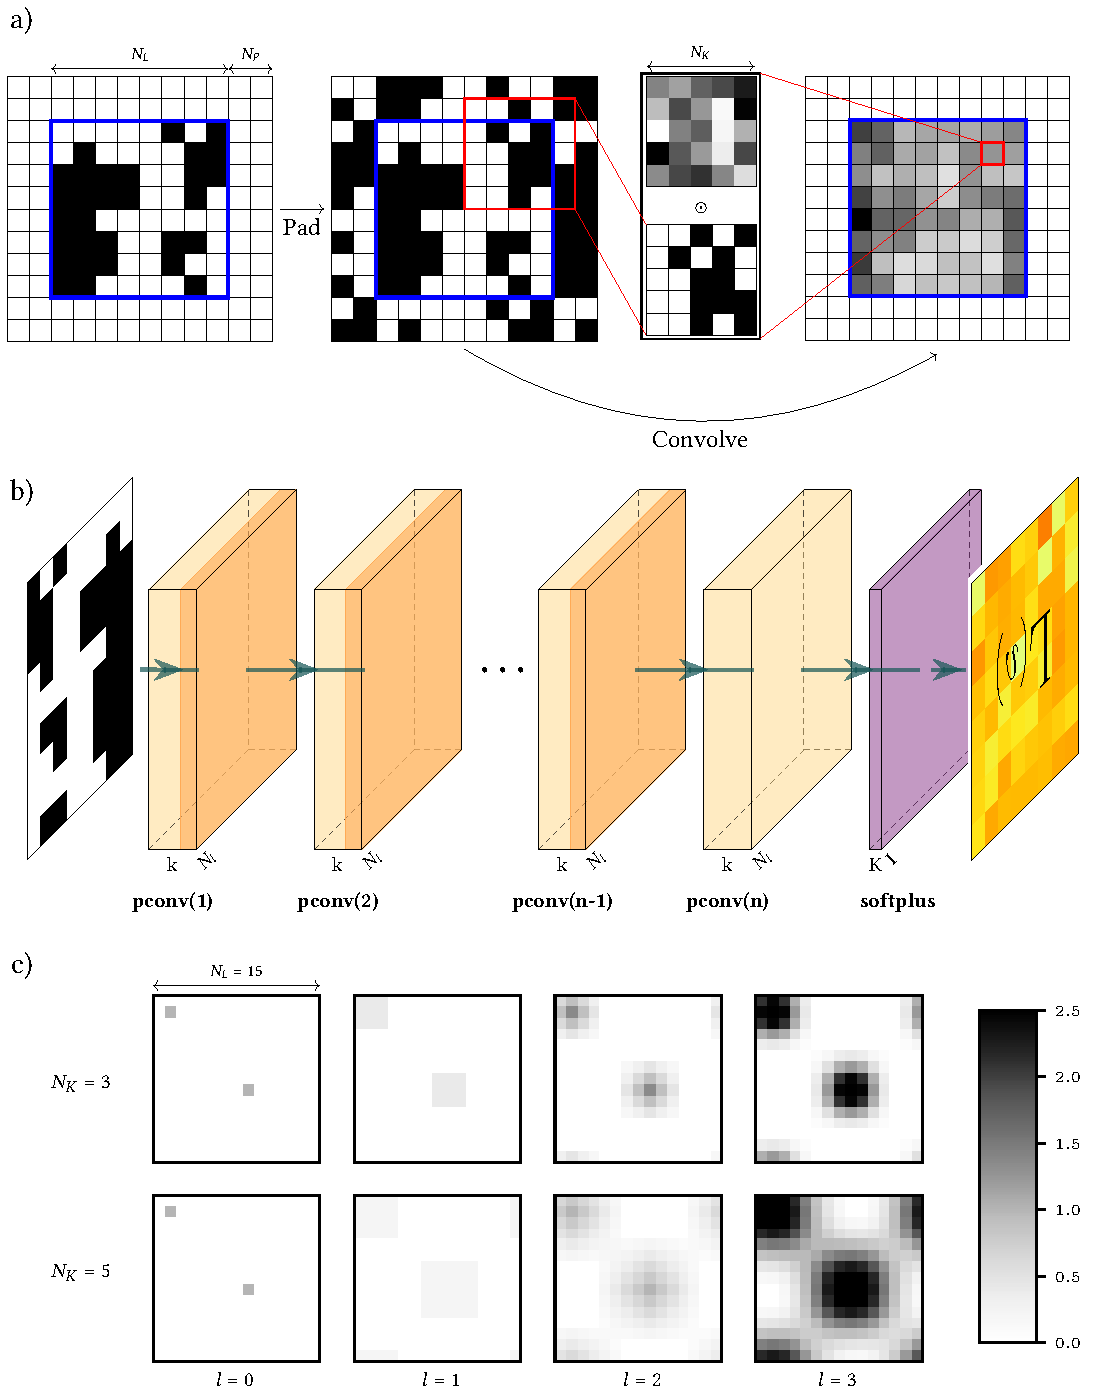
\includegraphics[width=\linewidth]{Chapter4/Figs/Vector/pcnn.pdf}
	\caption[Periodic CNN]{\textbf{Periodic CNN.} Each layer consists of periodic padding, and then convolving. The output shape matches the input shape (\textbf{top}). The pCNN architecture, takes state $s$ as input and outputs rates $\Gamma(s)$, similar to~\cite{gispen2020ground} (\textbf{middle}). While the receptive field of a single node is reduced in a CNN, faraway nodes are still connected indirectly after enough layers, how many layers depends on the kernel size and stride. Figure shows successive applications of the convolutional layers for $N_s=1$ and $N_K = 3$ or $N_K=5$, (\textbf{bottom}).}
	\label{fig:pcnn}
\end{figure}
\subsection{Group-Equivariant CNN}
The basic convolutional layer is translation equivariant, providing an advantage when we expect the same equivariant behaviour between the input and output. Alongside translational symmetry we can take advantage of other symmetries present in the lattice model. Recent work~\cite{bronstein2021geometric, cohen2016group} in the field of \textbf{geometric} deep learning has shown how to construct layers equivariant to arbitrary group symmetry, in the case of discrete grid-like data referred to as \textbf{group-equivariant} convolutional layers. At the core of {group convolution} is moving the filter using group action (rotation, translation, etc.). Adopting notation of Bronstein~\cite{bronstein2021geometric}, we write a group convolution as the inner product of the input $x$ and a filter transformed by group element $\mathfrak{g} \in \mathfrak{G}$ via group representation $\rho(\mathfrak{g})$ as $\rho(\mathfrak{g}) \theta_{u}=\theta_{\mathfrak{g}^{-1} u}$,
\begin{equation}
(x \star \theta)(\mathfrak{g})=\sum_{u \in \Omega} x_{u} \rho(\mathfrak{g}) \theta_{u}.
\end{equation}
\begin{figure}[h]
	\centering
	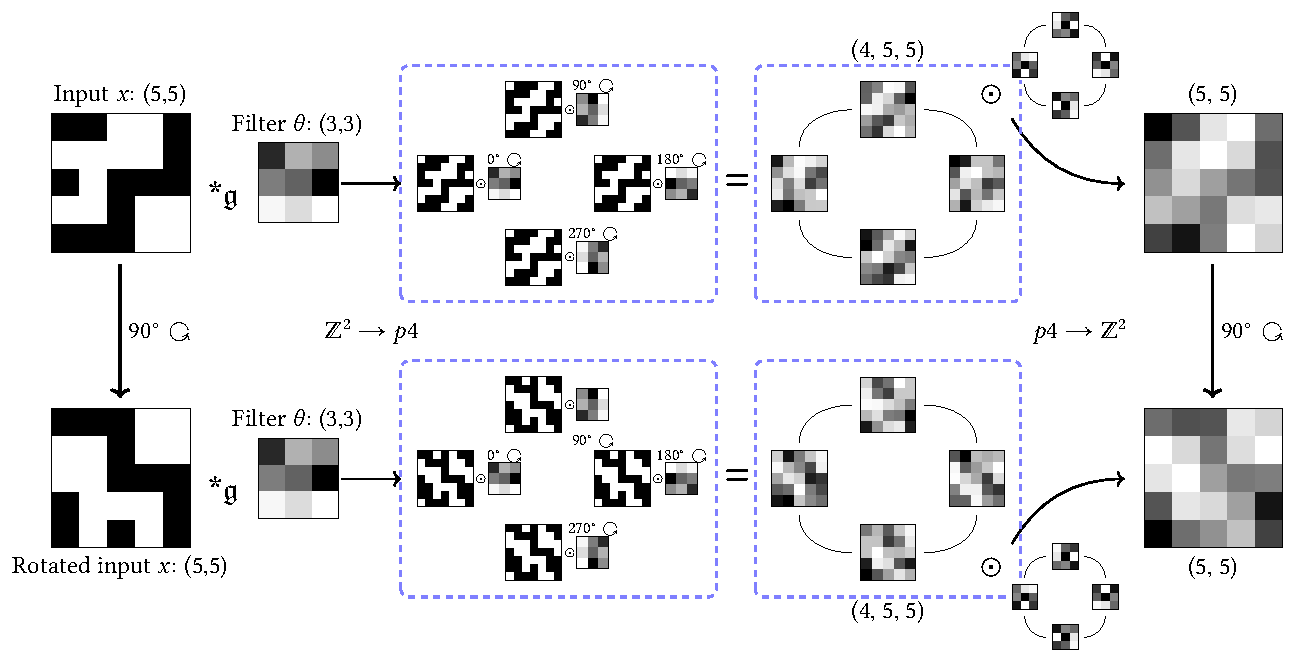
\includegraphics[width=\linewidth]{Chapter4/Figs/Vector/gcnn}
	\caption[Group-equivariant convolution]{\textbf{g-CNN layer.} Comparison of rotated inputs passing through two $p4$ equivariant layers. The first layer $\mathbb{Z}^2 \rightarrow p4$ produces a structured output, one convolution per each rotation of the filter $\theta$, the second layer $p4 \rightarrow \mathbb{Z}^2$ is an elementwise convolution between the structured output and rotations of the second filter. The layers are equivariant to $\frac{\pi}{2}$ rotation.}
	\label{fig:gcnn}
\end{figure}
We can separate the ordinary convolution from additional group transformations by writing a general group element $\mathfrak{g} \in \mathfrak{G}$ as a composition of a translation $\mathfrak{t}$ and rotation $\mathfrak{r}$, $\mathfrak g = \mathfrak{tr}$, and using  $\rho(\mathfrak{t r})=\rho(\mathfrak{t}) \rho(\mathfrak{r})$
\begin{equation}
	(x \star \theta)(\mathfrak{t r}) =\sum_{u \in \Omega} x_{u} \rho(\mathfrak{t}) \rho(\mathfrak{r}) \theta_{u} =\sum_{u \in \Omega} x_{u}(\rho(\mathfrak{r}) \theta)_{u-\mathfrak{t}},
\end{equation}
This yields a standard convolution with a transformed filter $\rho(\mathfrak{r})\theta$, meaning that we can implement the group-equivariant layer by first transforming the filter and performing convolution with each of these transformations, for details see Fig.~\ref{fig:gcnn} and~\cite{cohen2016group}.

\section{Gradient-based optimisation}
\label{sec:gbopt}

\subsection{Automatic differentiation}
\label{subsec:autodiff}
The demand for automatic evaluation of derivatives is today greater than ever, and automatic differentiation has seen wide adoption within the scientific computing and machine learning communities~\cite{baydin2018automatic, lyu2013automatic, tamayo2018automatic}, with the development of high profile libraries such as \emph{PyTorch}~\cite{paszke2017automatic}, \emph{TensorFlow}~\cite{abadi2016tensorflow}, or \emph{JAX}~\cite{jax2018github}. Not to be confused with numerical or symbolic differentiation, \textbf{automatic differentiation} (AD) provides a way to mechanically find derivatives of functions expressed as a computer program, with certain complexity guarantees~\cite{barak2016history}. While modern implementations employ a variety of tricks, AD has two basic \emph{modi operandi} of calculating partial derivatives of $f(x_1, x_2, \ldots, x_n): \mathbb{R}^n \rightarrow \mathbb{R}^m$ at $\mathbf{a}$. We start by representing the computation $y = f(\mathbf{x})$ as an \emph{evaluation trace} of elementary operations, composed of inputs, intermediate values, and outputs:
\begin{itemize}
	\item \textbf{Forward accumulation mode}~\cite{wengert1964simple}:  In forward mode, when evaluating the partial derivative w.r.t input $x_j$, we associate each intermediate value $v_i$ with the partial derivative $\frac{\partial v_i}{\partial x_j}$. We then apply the chain rule to each operation in the evaluation trace, producing the derivative trace. A single forward pass, in tandem passing both primals $v_i$ and their tangents $\frac{\partial v_i}{\partial x_j}$ through the trace, produces the output of the function, as well as the desired partial derivative. Forward mode AD produces one \emph{column} of the Jacobian $\textbf{J}_f$ at each pass, and is suited for functions with $n \ll m$.
	
	\item \textbf{Reverse accumulation mode}~\cite{speelpenning1980compiling}: In reverse mode, we associate each intermediate value $v_i$ with adjoint $\bar{v}_i = \frac{\partial y_i}{\partial v_i}$, partial derivative of the output $y_i$. Derivatives w.r.t inputs are then evaluated in a two step process. First, a forward pass populates intermediate values $v_i$ and stores their dependencies before the adjoints $\bar{v}_i$ are propagated in reverse, from outputs to inputs. Reverse mode AD produces one \emph{row} of the Jacobian $\textbf{J}_f$ at each pass, and is suited for functions with $n \gg m$.
\end{itemize}
AD is most commonly implemented in one of two ways, either by \emph{operator overloading}, abstracting away the derivative part of the calculation, e.g. in \emph{TensorFlow} of \emph{JAX}~\cite{abadi2016tensorflow, jax2018github}. Or alternatively via \emph{source code transformation}, where a new function is constructed by altering the source code, see \emph{Zygote}~\cite{innes2018don}.

\subsection{Optimisation algorithms}
Variants of the \textbf{stochastic gradient descent} (SGD) are by far the most used optimisation algorithms in ML. Instead of calculating the true gradient of the parameters w.r.t loss, it is estimated using an unbiased estimator which takes the average gradient on a minibatch of examples. SGD introduces only a single hyperparameter, the learning rate $\alpha$, which determines the size of correction $\theta \leftarrow \theta - \alpha \nabla_\theta L$ at each iteration. The main advantage of this approach is that the time complexity of an iteration does not depend on the number of examples. This is useful for cases with large, or even infinite in our case, training sets. The first improvement over vanilla SGD is the use of momentum~\cite{polyak1964some}, where an exponentially decaying average of past gradients determines the update direction. Second improvement is using an adaptive learning rate, \emph{ADAM}~\cite{kingma2014adam} is perhaps the most popular such algorithm. 

\section{Importance Sampling}
\label{sec:Impl-MCIP}
Ultimately we want to use the optimal learned rates $\Gamma^{(v)}$ to evaluate observables $\hat O$ in our model, be it the ground state energy or something else. Recall from section~\ref{sec:vmc}, that we can express observables as a Monte Carlo average of the local operator $\hat O_L$. But not all operators are made equal and some are more convenient to evaluate than others. In our implementation it will be helpful to make a distinction between \emph{diagonal} and \emph{off-diagonal} observables~\cite{torlai2018neural}. Since the wave functions of stoquastic Hamiltonians are real and positive, we denote $\psi(\boldsymbol{s}) = \sqrt{\rho(\boldsymbol{s})/Z}$, where $Z$ is the normalisation constant. If the observable
\begin{equation}
	\hat {O}=\sum_{\boldsymbol{s}, \boldsymbol{s}^{\prime}} {O}_{\boldsymbol{s} \boldsymbol{s}^{\prime}}|\boldsymbol{s}\rangle \langle \boldsymbol{s}^{\prime}|,
\end{equation}
is diagonal $\hat{O}_{\boldsymbol{s} \boldsymbol{s}^{\prime}}^{D}={O}(\boldsymbol{s}) \delta_{\boldsymbol{s} \boldsymbol{s}^{\prime}}$ in our chosen basis $\{\boldsymbol{s}\}$, then its expectation simplifies to 
\begin{equation}
	\langle\hat{O^D}\rangle=\sum_{\boldsymbol{s}, \boldsymbol{s}^{\prime}} \psi^*(\boldsymbol{s}) \psi(\boldsymbol{s}^{\prime}) {O}_{\boldsymbol{s} \boldsymbol{s}^{\prime}} = \frac{1}{Z} \sum_{\boldsymbol{s}} \rho(\boldsymbol{s}) O({\boldsymbol{s}})  \approx \frac{1}{M} \sum_{k=1}^{M} O(\boldsymbol{s}_{k}),
\end{equation}
which is very easy to evaluate given the MC samples. Alternatively for off-diagonal observables the expectation becomes
\begin{equation}
	\left\langle\hat{O}^{OD}\right\rangle=\sum_{\boldsymbol{s}, \boldsymbol{s}^{\prime}} \psi^{*}(\boldsymbol{s}) \psi(\boldsymbol{s}^{\prime}) O_{\boldsymbol{s} \boldsymbol{s}^{\prime}} = \frac{1}{\sum_{\boldsymbol{s}}\left|\psi_{\boldsymbol{\lambda}}(\boldsymbol{s})\right|^{2}} \sum_{\boldsymbol{s} \boldsymbol{s}^{\prime}} \psi_{\boldsymbol{\lambda}}^{*}(\boldsymbol{s}) \psi_{\boldsymbol{\lambda}}(\boldsymbol{s}^{\prime}) O_{\boldsymbol{s} \boldsymbol{s}^{\prime}} \approx \frac{1}{M} \sum_{k=1}^{M} O^L(\boldsymbol{s}_{k}),
\end{equation}
where the local operator has the form
\begin{equation}
	O_{\boldsymbol{s}_{k}}^{L}=\sum_{\boldsymbol{s}^{\prime}} \frac{\psi(\boldsymbol{s}^{\prime})}{\psi\left(\boldsymbol{s}_{k}\right)} O_{\boldsymbol{s}_{k} \boldsymbol{s}^{\prime}} = \sum_{\boldsymbol{s}^{\prime}} \sqrt{\frac{\rho(\boldsymbol{s}^{\prime})}{\rho\left(\boldsymbol{s}_{k}\right)}} O_{\boldsymbol{s}_{k} \boldsymbol{s}^{\prime}}. 
\end{equation}
The local estimate of $\hat{O}$ is efficient to evaluate if the matrix representation $O_{\boldsymbol{s}_{k} \boldsymbol{s}^{\prime}}$ is sparse in the reference basis. When working in the $z$-spin basis, an example of a diagonal observable would be the average longitudinal magnetisation per spin 
\begin{equation}
	\langle \hat \sigma_z \rangle = \sum_i \frac{\langle \hat \sigma^z_{i} \rangle}{N}.
\end{equation}
On the other hand, transverse magnetisation $\langle \hat \sigma^x_j \rangle$ for spin $j$ is off-diagonal\footnote{$\boldsymbol{s}_i = (s_1, s_2, \ldots, s_i, \ldots, s_n)$, $s_i$ is either $1$ or $0$.}
\begin{equation}
	\left\langle\boldsymbol{s}\left|\hat{\sigma}_{j}^{x}\right| \boldsymbol{s}^{\prime}\right\rangle=\delta_{s_{j}^{\prime}, 1-s_{j}} \prod_{i \neq j} \delta_{s_{i}^{\prime}, s_{j}},
\end{equation}
thus the local operator for $\langle \hat \sigma^x_j \rangle$ is sparse with only one term in the sum
\begin{equation}
	\left(\sigma_{j}^{x}\right)^{L}=\frac{\psi \left(s_{1}, \ldots, 1-s_{j}, \ldots, s_{N}\right)}{\psi\left(s_{1}, \ldots, s_{j}, \ldots, s_{N}\right)}=\sqrt{\frac{\rho \left(s_{1}, \ldots, 1-s_{j}, \ldots, s_{N}\right)}{\rho\left(s_{1}, \ldots, s_{j}, \ldots, s_{N}\right)}}.
\end{equation}

\subsection{MCMC and the Metropolis-Hastings Algorithm}
\label{subsec:Impl-MCMC}
The integration technique from the previous section relies on our ability to obtain samples from an unnormalised probability distribution $\rho$. \textbf{Markov Chain Monte Carlo} (MCMC) avoids sampling directly from $\rho$ by constructing a Markov chain, whose stationary distribution $\pi$ is the same as $\rho$. Propagating this chain produces a sequence of samples from the desired distribution. For the process to have a unique stationary distribution, it must be \emph{ergodic} and it must obey \emph{detailed balance}
\begin{equation}
	P_{\mathbf{s \rightarrow \mathbf{s}^\prime}}\rho(\mathbf{s}) = P_{\mathbf{s^\prime \rightarrow \mathbf{s}}} \rho(\mathbf{s}^\prime),
\end{equation}
where $P$ are transition probabilities. The equivalent condition in continuous time uses the rate matrix $\Gamma$
\begin{equation}
	\Gamma_{\mathbf{s \rightarrow \mathbf{s}^\prime}}\rho(\mathbf{s}) = \Gamma_{\mathbf{s^\prime \rightarrow \mathbf{s}}} \rho(\mathbf{s}^\prime).
\end{equation}
The \emph{correct} transition probabilities $P$ (or rates $\Gamma$) are not known, instead each move is proposed using a trial move probability $T_{\mathbf{s \rightarrow \mathbf{s}^\prime}}$ and accepted using the Metropolis-Hastings acceptance probability $A_{\mathbf{s \rightarrow \mathbf{s}^\prime}}$ which guarantees detailed balance is met
\begin{equation}
	A_{\mathbf{s \rightarrow \mathbf{s}^\prime}} = \min \left(1, \frac{T_{\mathbf{s^\prime \rightarrow \mathbf{s}}} \rho(\mathbf{s}^\prime)}{
		T_{\mathbf{s \rightarrow \mathbf{s}^\prime}}\rho(\mathbf{s})}\right).
\end{equation} 
Thus to sample from any probability distribution we only need the ability to calculate ratios $\frac{\rho(\boldsymbol{s}^{\prime})}{\rho(\boldsymbol{s})}$ and to sample from a trial transition probability $\mathrm T_{\mathbf{s \rightarrow \mathbf{s}^\prime}}$. The efficiency of the algorithm depends on the amount of trial moves that we reject and accepting every trial move would mean \textbf{optimal importance sampling}. All moves are accepted only when $T = P$, which would just mean sampling from $\mathrm P$ directly. 

In practice we are interested in sampling from the ground state $\psi_0$, and we can improve upon the standard method of using uniform transition probabilities for all adjacent states, by recalling that sampling from the Feynman-Kac $\mathbb{P}_\text{FK}$ measure is equivalent to sampling from the ground state. Thus it is possible to achieve optimal importance sampling by finding the rates $\Gamma^\prime$ that correspond to the Feynman-Kac measure, which is precisely what we discussed in section~\ref{sec:control_loss}. This is possible in theory, but our variational approximation of the rates $\Gamma^{\theta} \approx \Gamma^\prime$ is not exact in the same way that a trial wave function is not, and we are really sampling from the stationary distribution of $\Gamma^\theta$. The actual sampling of the chain can be done in discrete time, using
\begin{equation}
	T_{s \rightarrow s^{\prime}}=\frac{\Gamma_{s \rightarrow s^{\prime}}^{\theta}}{\sum_{s^{\prime} \neq s} \Gamma_{s \rightarrow s^{\prime}}^{\theta}}
\end{equation}
and a Metropolis correction step\footnote{Throwing away holding times $\tau_i$ biases the chain.} with ${\frac{\rho\left(\boldsymbol{s}^{\prime}\right)}{\rho(\boldsymbol{s})}} = \frac{\Gamma_{s \rightarrow s^{\prime}}}{\Gamma_{s^{\prime} \rightarrow s}}$. Alternatively it can be done in continuous time, where the stationary distribution $\rho = \left[ \tilde{\rho_1}, \tilde{\rho_2}, \tilde{\rho_3}, \ldots \right]$, where $\tilde \rho_i$ is the fraction of time spent in state $i$.

\section{Software implementation details}
\label{sec:qoptsampl}
The main developing principles for the implementation are flexibility in the choice of variational model, hyperparameters, or stoquastic Hamiltonian itself, and extendability, the ability to add new Hamiltonians and models with relative ease. Additionally, the implementation needs to be computationally efficient with its most demanding parts running on the GPU. This sort of dichotomy between flexibility and speed is aided by modern ML frameworks. We work in \emph{JAX}~\cite{jax2018github} which extends \emph{numpy} with \emph{function transformations}, provides automatic differentiation capabilities and uses just-in-time\footnote{It uses the \emph{Accelerated Linear Algebra} XLA compiler.} (jit) compilation to improve performance. The design of the implemented software is shown in Fig.~\ref{fig:qsampl}. Since the workflow of the method is split between training and sampling, so is the software.

The \textbf{input layer} includes the implementation of a Stoquastic Hamiltonian, which must include methods for calculating the passive rates, potential, adjacent states, and for transforming one adjacent state into another. The variational module must be a subclass of \emph{flax.linen.Module} and returns $\Gamma_{s\rightarrow s^\prime}$ for input $s$. All parameters are taken as an \emph{.ml\_collections} dictionary.

The \textbf{training layer}, takes the input functions and partially compiles them for the input parameters before performing training. The most important part of the training procedure is the generation of a batch of trajectories. This can be performed in a number of ways, so long as all trajectories have constant $T$ and fixed endpoints. The generation is system dependent, and we propose the following three approaches for the TFIM model, where spin flips are independent. 
\begin{enumerate}[label=\roman*)]
	\item \textbf{Permute:} This is the simplest batch generation technique. First a single trajectory is obtained and is stored as holding times $\tau_i$ and actions $a_i$, along with the initial state $S_0$. Then the times and actions are permuted into a batch of $N_b$ permutations. The choice of initial trajectory is arbitrary, current implementation supports sampling it from the latest rates $\Gamma^{v_i}_{s \rightarrow s^\prime}$, passive rates, or the initial rates $\Gamma^{v_0}_{s \rightarrow s^\prime}$. The problem with \emph{permute} batch generation is that the number of actions is constant, and this may pose problems as discussed in~\ref{subsec:elusive_lambda}.
	
	\item \textbf{Split:} Batch generation using the \emph{split} method also relies on sampling an initial trajectory before modifying it. Instead of only permuting the original, we now append two flips of a randomly chosen spin to the trajectory before shuffling. This has no bearing on the endpoints of the trajectory but changes its length\footnote{Length refers to number of spin flips not $T$.}. The times can be resampled or a random holding time can be split among the new visited states, so that all trajectories in the batch have constant $T$.
	
	\begin{figure}[H]
		\centering
		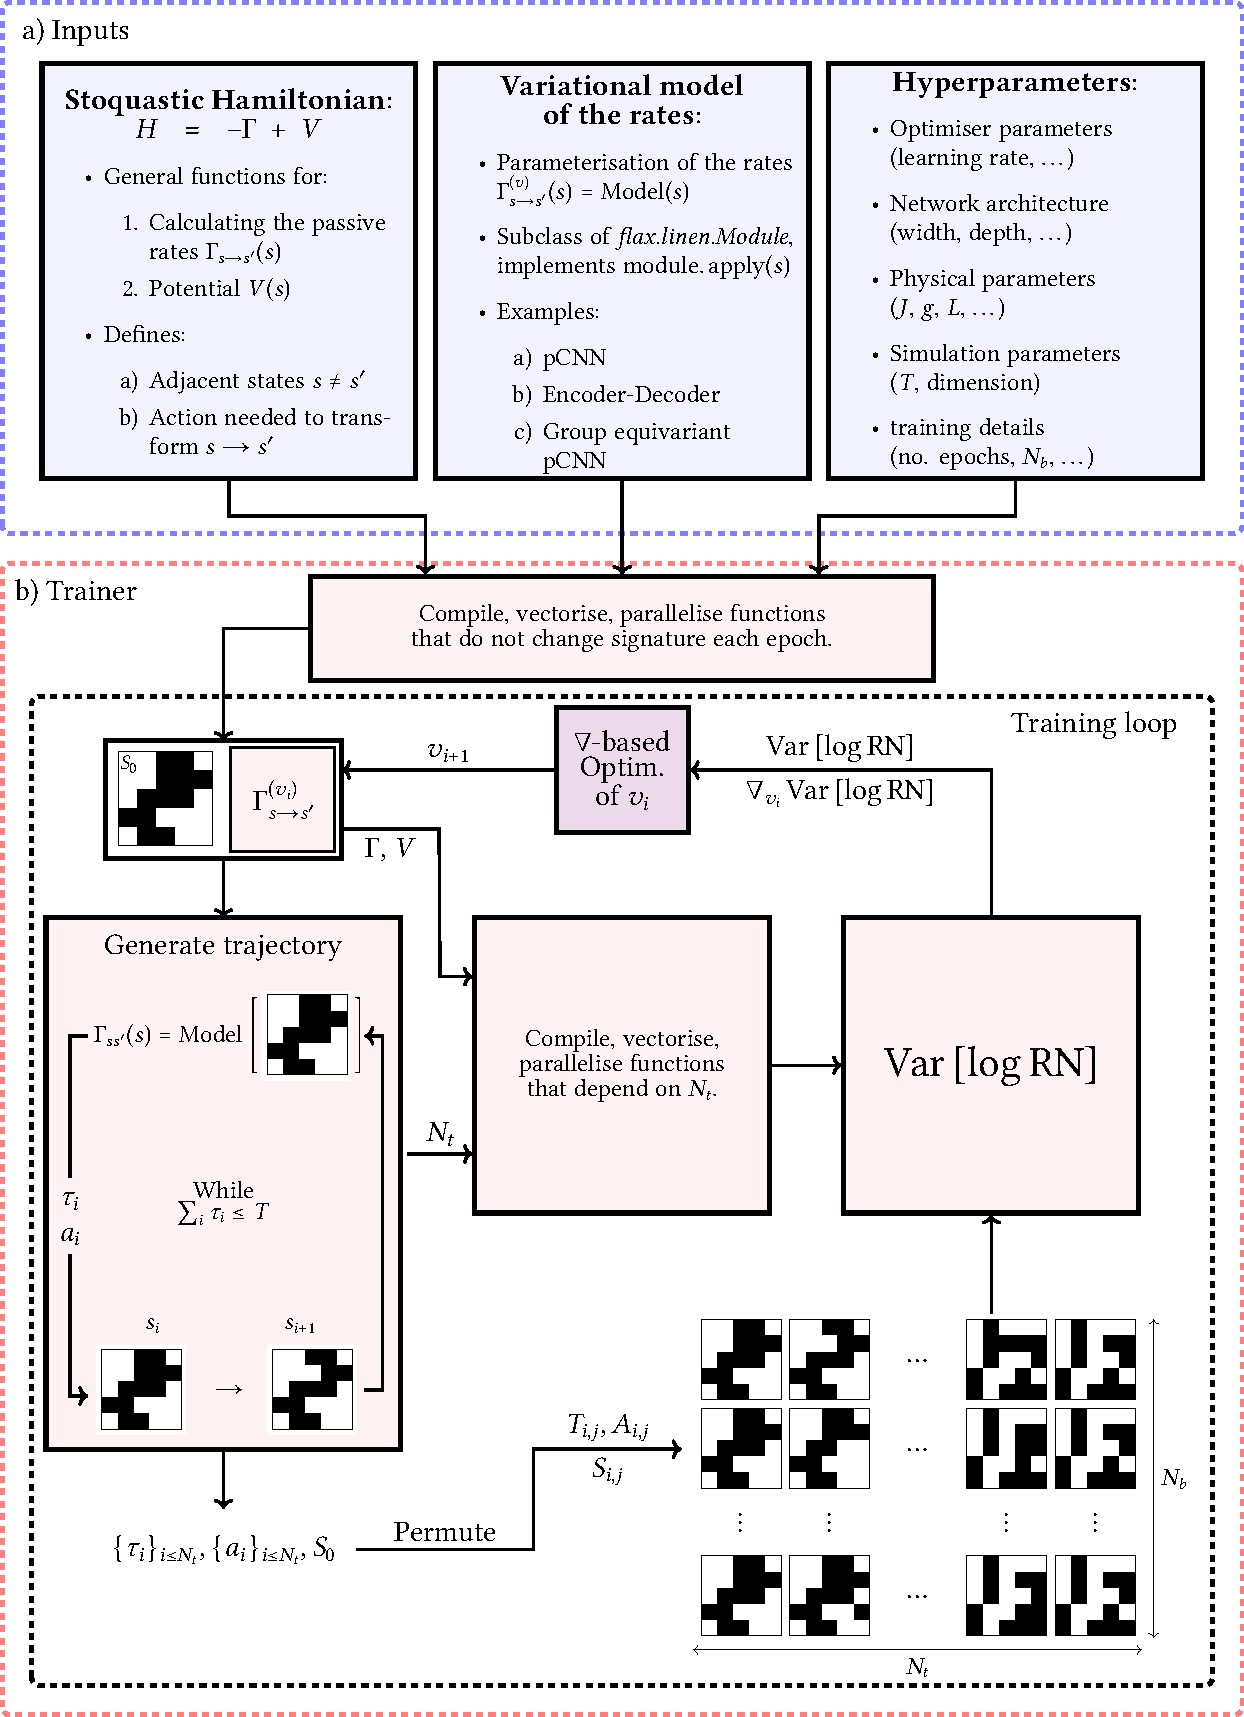
\includegraphics[width=\linewidth]{Chapter4/Figs/Vector/qsampl1}
	\end{figure}
	\begin{figure}[t!]
		\ContinuedFloat
		\centering
		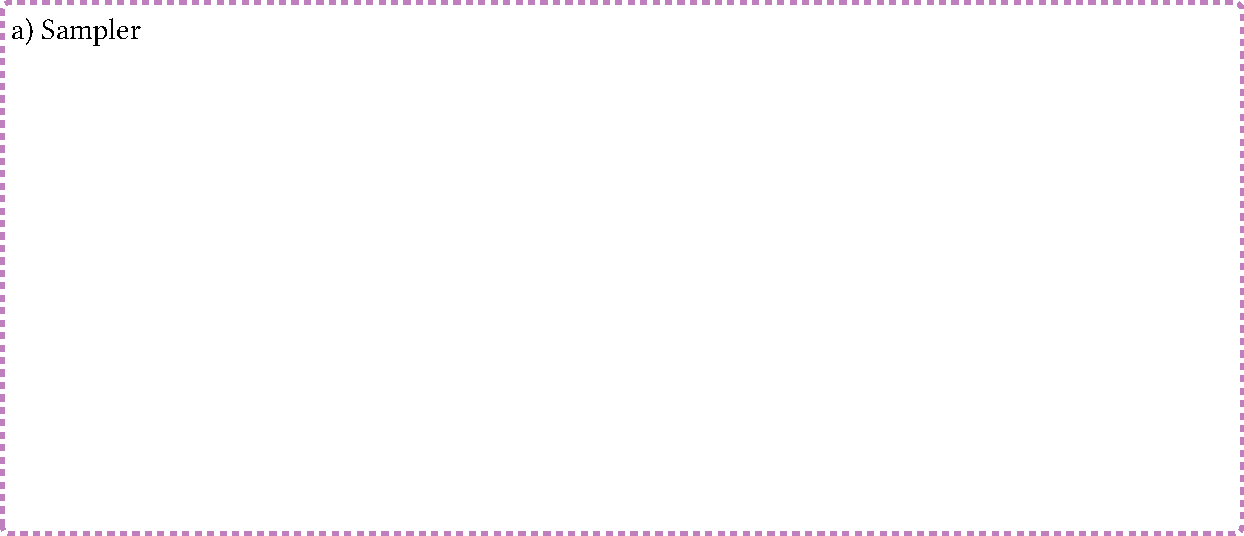
\includegraphics[width=\linewidth]{Chapter4/Figs/Vector/qsampl2}
		\caption[Implementation details]{\textbf{Software implementation details.} The software implementation in JAX is divided into three layers. The input layer (\textbf{a}) specifies the Hamiltonian for which we are learning the rates, the model used to represent the rates and training hyperparameters. The trainer layer (\textbf{b}) specialises the general functions for the system at hand and training details (batch size, time, etc.), before training the rates and outputing a sampler object. The sampler object (\textbf{c}) can then be used to perform importance sampling using the trained rates in either discrete or continuous time, if operators are provided observables can be evaluated while sampling a trajectory.}
		\label{fig:qsampl}
	\end{figure}
	
	\item \textbf{Construct:} The \emph{construct} method does not sample any trajectory. It exploits the fact that if we assign each spin an odd or even number of flips, we obtain a family of trajectories with fixed endpoints. We first randomly choose $N_a$ spins, which will be flipped during the trajectory. Of these spins, we then mark $N_e$ spins to be even and the rest to be odd. To obtain a batch of trajectories with variable length, we assign different odd numbers of flips to odd spins, and analogous to even flips. The times are sampled independently from an exponential distribution and normalised to add up to desired $T$. The benefit of this method is that we can have trajectories of very different length in the same batch.
\end{enumerate}
The gradient of the $\log RN$ loss is then evaluated using an MC estimate and the parameters updated accordingly, the implementation only supports the \emph{ADAM} optimiser. 

The \textbf{sampling layer} is essentially a wrapper that provides a friendly way of working with the learned rates. It implements functionality for sampling with rates in parallel, either in discrete or continuous time, as well as evaluation diagonal and off-diagonal observables. The sampling from a CTMC can be done with one of two implemented methods
\begin{enumerate}[label=\roman*)]
	\item \textbf{Max step (competing exponentials):} For all adjacent states sample a holding time $\tau_i \sim \operatorname{Exp}(\lambda_i)$, then move into the state with the minimum time $\tau_i$.
	\item \textbf{Gumbel step:} The minimum of $n$ independent exponential distributions $\{\lambda_1, \lambda_2, \cdots, \lambda_n\}$ is also exponentially distributed with rate $\lambda = \sum_i \lambda_i$, its minimizer is distributed according to a multinomial distribution with $\pi_i =\frac{\lambda_{i}}{\lambda_{1}+\cdots+\lambda_{n}} $ and independent of time. We first sample a holding time $\tau$ from the exponential distribution and then the index from the multinomial.
\end{enumerate}
